\epigraph{The Babel fish is small, yellow, leech-like, and probably the oddest
thing in the universe. It feeds on brainwave energy  ...
%absorbing all unconscious
%frequencies and then excreting telepathically a matrix formed from the conscious
%frequencies and nerve signals picked up from the speech centres of the brain,
%the practical upshot of which is that 
if you stick a Babel fish in your ear, you can
instantly understand anything in any form of language.}{{\it The Hitchhiker's
Guide to the Galaxy}.
Douglas Adams.}
Human languages are diverse and rich in categories with about 6000 to 7000
languages spoken worldwide.\footnote{\url{http://www.linguisticsociety.org/content/how-many-languages-are-there-world}}
As civilization advances, the need for seamless communication and understanding across
languages becomes more and more crucial. Machine translation (MT), the
task of teaching machines to learn to translate automatically across languages, as
a result, is an important research area.
MT has a long history \cite{hutchins07} from the original
phiosophical ideas of universal languages in the seventeen century to the 
first practical instances of MT in the twentieth century, e.g., one proposal by
\newcite{weaver49}. Despite several excitement moments that led to hopes that MT
will be solved ``very soon'', e.g., the 701 translator\footnote{\url{http://www-03.ibm.com/ibm/history/exhibits/701/701_translator.html}}
developed by scientists at George Town and IBM in the 1950s or a simple
vector-space transformation
technique\footnote{\url{https://www.technologyreview.com/s/519581/how-google-converted-language-translation-into-a-problem-of-vector-space-mathematics/}} proposed by Google researchers at the beginning of the twenty-first
century,
MT remains to be an extremely challenging
problem.\footnote{\url{http://www.huffingtonpost.com/nataly-kelly/why-machines-alone-cannot-translation_b_4570018.html}}
To understand why MT is difficult, let us trace through one ``evolution''
path of % development
MT which crosses through techniques that are used extensively in
commercial MT systems. 

\begin{figure}
\centering
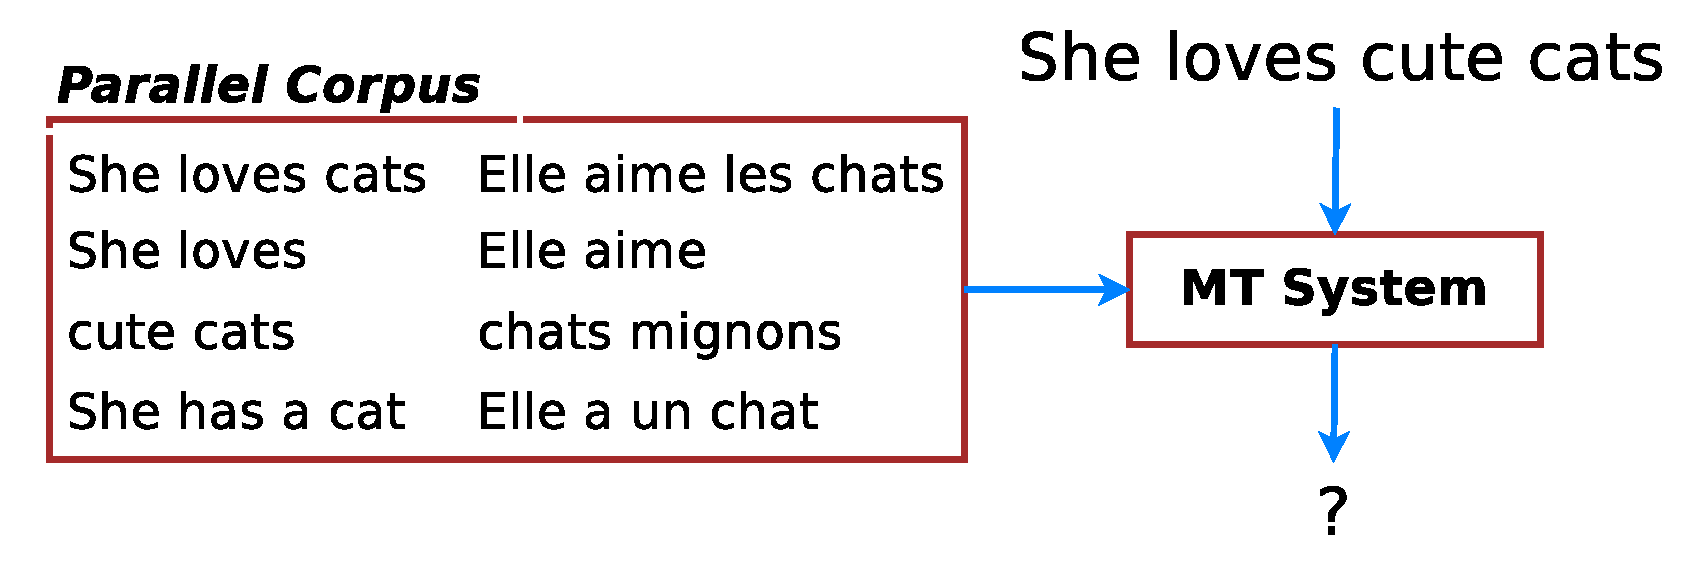
\includegraphics[width=0.6\textwidth, clip=true, trim= 0 0 0 0]{img/mt} % , angle=-90
\caption{{\bf Machine translation} (MT) -- a general setup of MT. Systems
build translation models from parallel corpora to translate new unseen
sentences, e.g., \word{She loves cute cats}.}
\label{f:mt}
\end{figure}

Modern
statistical MT started out with a seminal work by IBM scientists
\cite{Brown:1993:MSM}. The proposed technique requires minimal linguistic
content and only needs a {\it parallel corpus}, i.e., a set of pairs of sentences that are translations of one
another, to train machine learning algorithms to tackle the translation problem.
Such a language-independent setup is illustrated in Figure~\ref{f:mt} and remains
to be the general approach for nowadays MT systems.
For over twenty years since the IBM seminal paper, approaches in MT
such as
\cite{Koehn:2003:SMT,och03,Liang:2006:EDA,koehn2007moses,chiang07hiero,dyer10cdec,cer10phrasal},
%inter alia, 
are, by and large, similar according to the following two-stage
process (see Figure~\ref{f:phrase_mt}). First, source sentences are broken into
chunks which can be translated in isolation by looking up a ``dictionary'', or
more formally a {\it translation model}. Translated target words and phrases
are then put together to form coherent and natural-sounding sentences by consulting a
{\it language model} (LM) on which sequences of words, i.e., {\it \ngram{}s}, are
likely to go with one another.

\begin{figure}[tbh!]
\centering
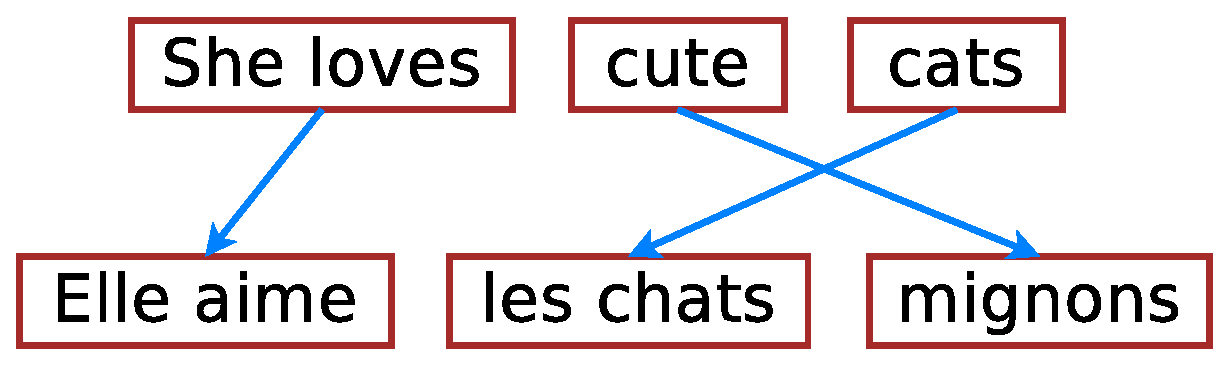
\includegraphics[width=0.45\textwidth, clip=true, trim= 0 0 0 0]{img/phrasemt} % , angle=-90
\caption{{\bf Phrase-based machine translation} (MT) -- example of how phrase-based
MT systems translate a source sentence \word{She loves cute cats} into a target sentence
\word{Elle aime les chats mignons}: sentences are split into chunks and phrases
are translated.
} 
\label{f:phrase_mt}
\end{figure}

The aforementioned approach, while has been successfully deployed in many commercial systems,
does not work very well and suffers from the following two major drawbacks.
First, translation decisions are {\it locally determined} as we translate
phrase-by-phrase and long-distance dependencies are often ignored. Second, it is
slightly ``strange'' that language models (LMs), despite being a key component in the MT
pipeline, utilize context information that is both short, consisting of only
a handful of previous words, and target-only, never looking at the source
words. These shortcomings in LMs gives rise to a new wave of {\it hybrid} systems which
aim to empower phrase-based MT with neural network components, most notably
neural language models (NLMs). 

NLMs were first proposed by \newcite{Bengio2003}
as a way to combat the ``curse'' of dimensionality suffered by traditional LMs.
In traditional LMs, one has to explicitly store and handle 
all possible \ngram{}s occurred in a training corpus, the number of which
quickly becomes enormous. As a result, existing MT systems often limit
themselves to use only short, e.g., $5$-gram, LMs \cite{kenlm}, which capture little context
and cannot generalize well to unseen \ngram{}s. NLMs address these concerns by
using distributed representations of words and not having to explicitly store
all enumerations of words. As a result, many MT systems, \cite{schwenk07,vaswani13decode,luong15nlm}, inter
alia, start adopting NLMs alongside with traditional LMs.
To make NLMs even more powerful, recent work \cite{Schwenk12continuous,devlin14}
propose to condition on source words beside the target context to lower
uncertainty in predicting next words (see Figure~\ref{f:nnjm}).\footnote{In
\cite{devlin14}, the authors have constructed a model that conditions on 3
target words and 11 source words, effectively building a $15$-gram LM.}
\begin{figure}[tbh!]
\centering
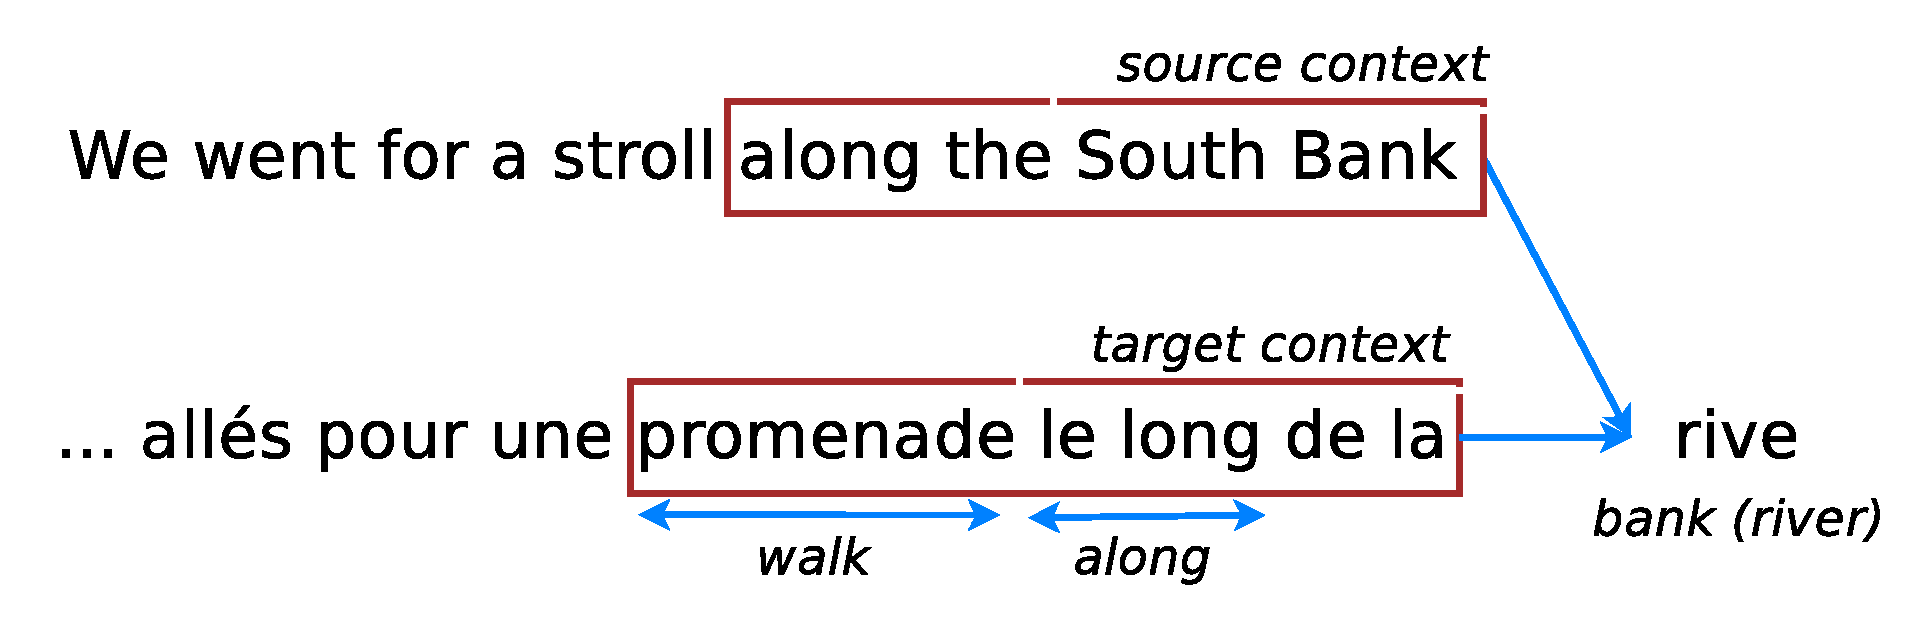
\includegraphics[width=0.7\textwidth, clip=true, trim= 0 0 0 0]{img/nnjm} % , angle=-90
\caption{{\bf Source-conditioned neural language model} (NLM) -- example of a source-conditioned
NLM proposed by \newcite{devlin14}. To evaluate a how likely a next word
\word{rive} is, the model not only relies on previous target words (context)
\word{promenade le long de la} as in
traditional NLMs \cite{Bengio2003}, but also utilizes source context \word{along the
South Bank} to lower uncertainty in its prediction.
} 
\label{f:nnjm}
\end{figure}

These hybrid MT systems with NLM components, while having addressed shortcomings
of traditional phrase-based MT,
still translate locally and fail to capture long-range dependencies. For example, in Figure~\ref{f:nnjm}, the
source-conditioned NLM does not see the word \word{stroll}, or any other words
outside of its fixed context windows, which can be useful in deciding that the
next word should be \word{bank} as in \word{river bank} rather \word{financial
bank}. More problematically, the entire MT pipeline is already complex with
different components needed to be tuned separatedly, e.g., translation models,
language models, reordering models, etc.; now, it becomes even worse as
different neural components are incorporated. Neural Machine Translation to the
rescue!


Neural Machine Translation (NMT) is a new approach to translating text from one
language into another that captures long-range dependencies in sentences and
generalizes better to unseen texts. The core of NMT is a single deep neural
network with hundreds of millions of neurons that learn to directly map source
sentences to target sentences. Despite being relatively new 
\cite{kal13,sutskever14,cho14}, NMT has already shown promising results,
achieving state-of-the-art performances for
several language pairs such as
English-French \cite{luong15}, English-German
\cite{jean15,luong15attn,sennrich16mono}, and
English-Czech \cite{jean15wmt,luong16}. 
NMT is appealing since it is conceptually
simple and can be trained
end-to-end. NMT translates as follows: it reads through the given source
words one by one until the
end, and then, starts emitting one target
word at a time until a special end-of-sentence symbol is produced. We illustrate
this process in Figure~\ref{f:nmt}. 
% for the model described in \cite{sutskever14}.

\begin{figure}[tbh!]
\centering
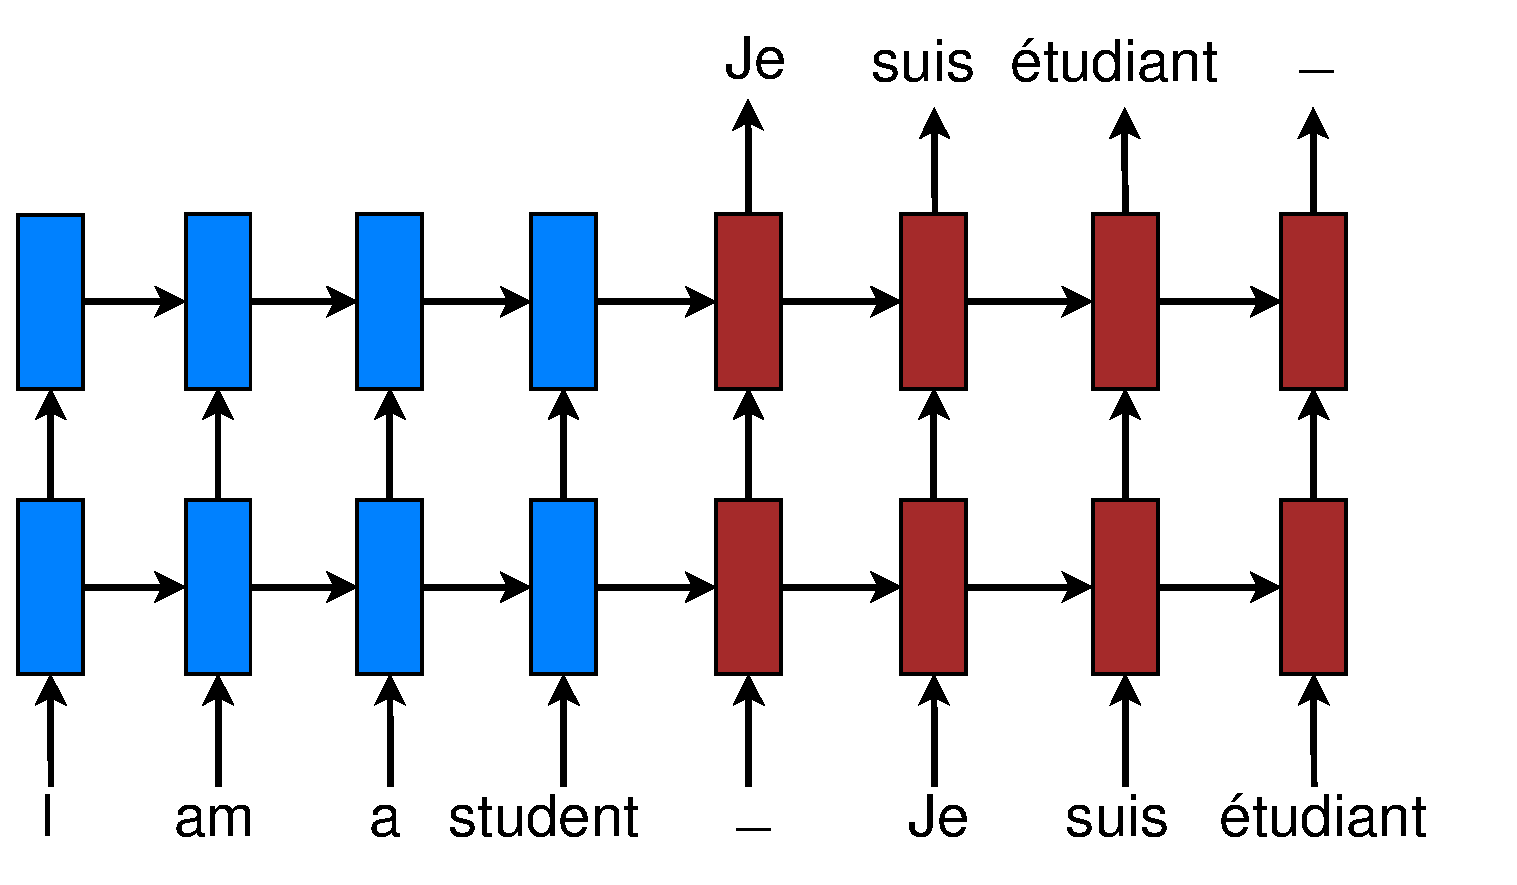
\includegraphics[width=0.6\textwidth, clip=true, trim= 0 0 0 0]{img/nmt_basic} % , angle=-90
\caption{{\bf Neural machine translation} -- example of a deep recurrent
architecture proposed by \newcite{sutskever14} for
translating a source sentence \word{I am a student} into a target sentence
\word{Je suis \'{e}tudiant}. Here, \word{\texttt{\_}} marks the end of a sentence.
} 
\label{f:nmt}
\end{figure}

Such simplicity leads to several advantages. 
NMT requires minimal domain knowledge: it only assumes access to
sequences of source and target words as training data and learns to directly
map one into another. NMT beam-search decoders that
generate words from left to right can be easily implemented, unlike the highly
intricate decoders in standard MT \cite{Koehn:2003:SMT}. Lastly, the use of
recurrent neural networks (RNNs) allow NMT to generalize well to very long word
sequences while not having to 
explicitly store any gigantic
phrase tables or language models as in the case of standard MT.

In this thesis, I will describe how I have pushed the limits of NMT, making it
applicable to a wide variety of languages with state-of-the-art performance.
We start off by providing background knowledge on RNN and NMT
in Chapter~\ref{c:background}. The following chapters detail my contributions.
Chapter~\ref{c:copy} discusses how the rare word
problem in NMT is addressed with a mechanism to ``copy'' words from source to
target; hence, extending the vocabulary
coverage. Chapter~\ref{c:attention} describes
how the attention mechanism, a way to select
local contexts in the source sentence as we transate, can be effectively used in
NMT to better handle long sentences. Chapter~\ref{c:hybrid} 
proposes a novel way of dealing with language complexity (rich morphology,
neologisms, and informal spellings) by building a hybrid word and character
level model which can gain from the flexibility of a character-level model while
maintaining the speed and quality of the word-level model. Towards the future of
NMT, I answer two questions in Chapter~\ref{c:future}: (1) whether we can improve translation by jointly
learning from a wide variety of sequence-to-sequence tasks such as parsing,
image caption generation, and auto-encoders or skip-thought vectors; and (2)
whether we can compress NMT for mobile devices.
Chapter~\ref{c:conclude} wraps up and discusses remaining challenges in NMT
research.
